\documentclass[a4paper,twoside]{article}

%% Language and font encodings
\usepackage[spanish]{babel}
\usepackage[utf8]{inputenc}
\usepackage[T1]{fontenc}


%% Sets page size and margins
\usepackage[a4paper,top=3cm,bottom=2cm,left=2.5cm,right=2.5cm,marginparwidth=0.5cm]{geometry}

\usepackage{amsmath}			%Paquete matemático
\usepackage{graphicx}
\usepackage[colorinlistoftodos]{todonotes}

\usepackage{hyperref}		%Paquete empleado para colocar hipervinculos
\hypersetup{
	colorlinks = true,
	linkcolor = black,
}

\usepackage{eurosym}
\usepackage{pdfpages}			%Sirve para incluir PDF en el documento
\usepackage{anysize}			%Podremos colocar imagenes de cualquier tamaño
\usepackage{subfig}				%Nos permitira colocar varias imagenes en una figura
\usepackage{float}				%Podremos crear y colocar boxes donee queramos
\usepackage[export]{adjustbox}

%Colocamos cabeceras y pies de pagina
%(CONSULTA: http://edicionesoniricas.com/maquetar-latex-encabezados-pies-pagina/)
%(CONSULTA2: https://es.sharelatex.com/learn/Headers_and_footers)
%\bfseries es análogo a \textbf{}
% \leftmark-> Adds name and number of the current top-level structure (section for article) in uppercase letters.
%\rightmark-> Adds name and number of the current next to top-level structure (subsection for article) in uppercase letters.
\usepackage{fancyhdr}		%Paquetes necesarios
\pagestyle{fancy}			%Borra los parametros por defecto
\fancyhf{}
\fancyhead[RO,LE]{\bfseries\thepage}
\fancyhead[LO,RE]{\bfseries\rightmark}
%Nos aseguramos de que en las paginas plain, no haya ni cabeceras ni lineas
\fancypagestyle{plain}
{
	\fancyhead{} % elimina cabeceras en paginas "plain"
	\renewcommand{\headrulewidth}{0pt} % así como la raya
}

%Definimos las lineas divisoras de las cabeceras y pie de pagina
\renewcommand{\headrulewidth}{1pt}	%Define el grosor de la línea de head
\renewcommand{\footrulewidth}{0pt}		%Define el grosor de la linea foot (Si no queremos linea, 0pt)
\addtolength{\headheight}{0.5pt} % espacio para la raya

%Librerias para introducir código de Matlab
%\usepackage{bigfoot} % to allow verbatim in footnote
\usepackage[numbered,framed]{matlab-prettifier}
\usepackage{listings,lstautogobble}
\lstset{
	style              = Matlab-editor,
	basicstyle         = \mlttfamily,
	escapechar         = ",
	mlshowsectionrules = true,
	autogobble=true
}

% Pie de pagina
%\fancyfoot{} % limpia el pie
\fancyfoot[C]{- \thepage -} % número de página centrado

%Nos generará texto para pruebas de maquetado
\usepackage{lipsum}

% Se varia el limite de colimnas de latex
\setcounter{MaxMatrixCols}{11}
\usepackage{lscape}
%----------------------------------------------------------------------------------------------------------------------------------
\begin{document}
\begin{titlepage}
	\centering
\Huge{\textbf{CONTROL Y PROGRAMACIÓN DE ROBOTS}} \\
\Huge{\textit{Proyecto de robótica móvil}}\\

\vspace{1cm}
\LARGE{Grado en Ingeniería Electrónica, Mecatrónica y Robótica}\\
\rule{\textwidth}{0.1mm}
%  %%%%% Este trozo de codigo es para insertar imagenes %%%%%%%
\begin{figure}[h!]
	\centering
	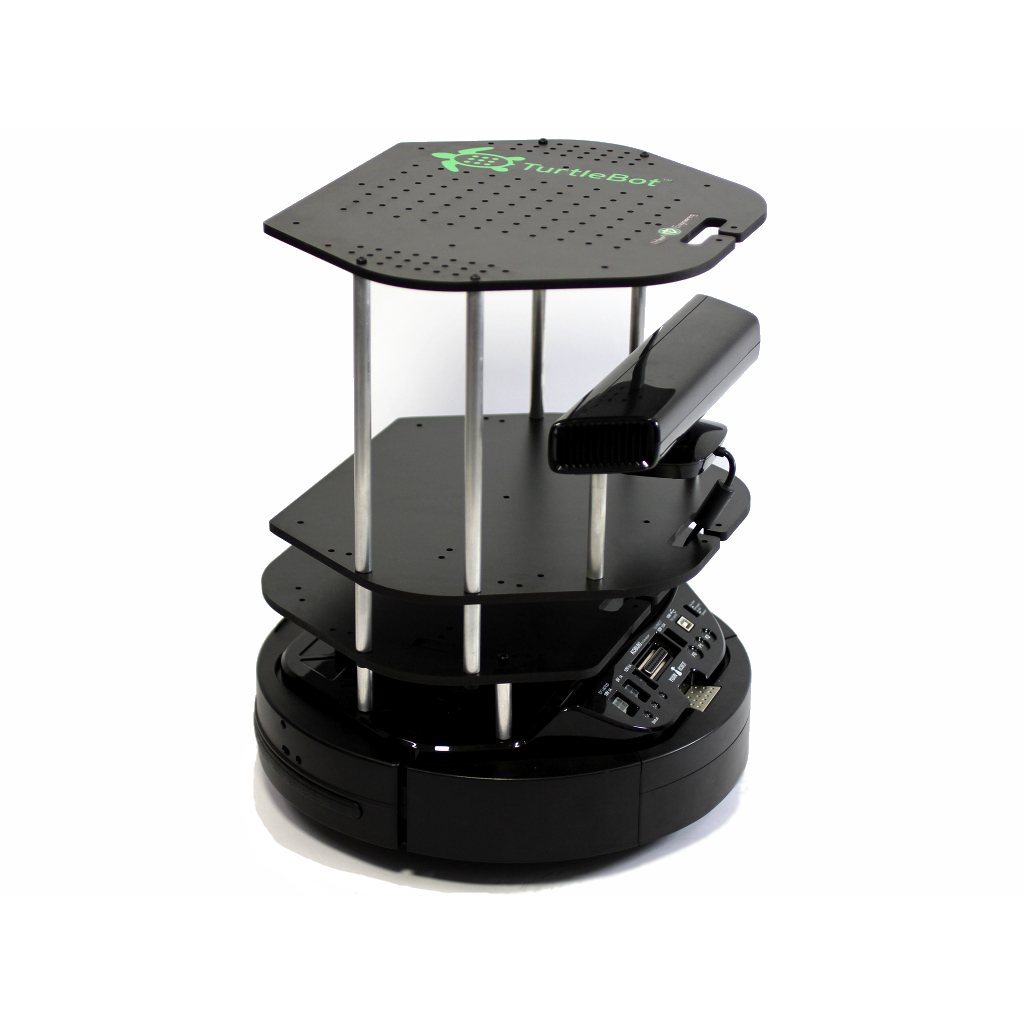
\includegraphics[width=.7\textwidth]{robot_portada}
	%\caption{textodelaleyenda}
\end{figure}
% %%%%%%%%%%%%%%%%%%%%%%%%%%%%%%%%%%%%%%%%%%%%%%%%%%%%%%%%%%%%%
\vspace{1cm}
\rule{\textwidth}{0.1mm}
\Large{\textbf{Autores:} Montes Grova, Marco Antonio\\
 Lozano Romero, Daniel\\
 Mérida Floriano, Javier}
\end{titlepage}
\tableofcontents
\newpage
% %%%%%%%%%%%   INTRODUCCION %%%%%%%%%%%%%%%%%%
\section{Introducción al proyecto}
En el proyecto que sigue a continuación se desarrollará el modelado y control de un robot móvil tipo síncrono. La principal característica destacable de este tipo de robots recae en el mecanismo mecánico interno que posee mediante el cuál se podrán mover 3 ruedas empleando únicamente 2 motores.\\
Con uno de los motores se desplazará en línea recta y con el otro se le dará el ángulo de giro deseado sobre sí mismo.\\

El modelo síncrono se basa en 3 ruedas idénticas que se desplazan y giran al unísono, haciendo posible que el robot pueda moverse en cualquier dirección y orientación en el plano del suelo. Estas ruedas están dispuestas de forma triangular en la base del robot, el cual se va a representar como un objeto cilíndrico, siendo la base uno de los lados circulares. Par un mayor entendimiento, se va a representar un esquema del mecanismo utilizado en este tipo de robot móvil:\\

\begin{figure}[h!]
	\centering
	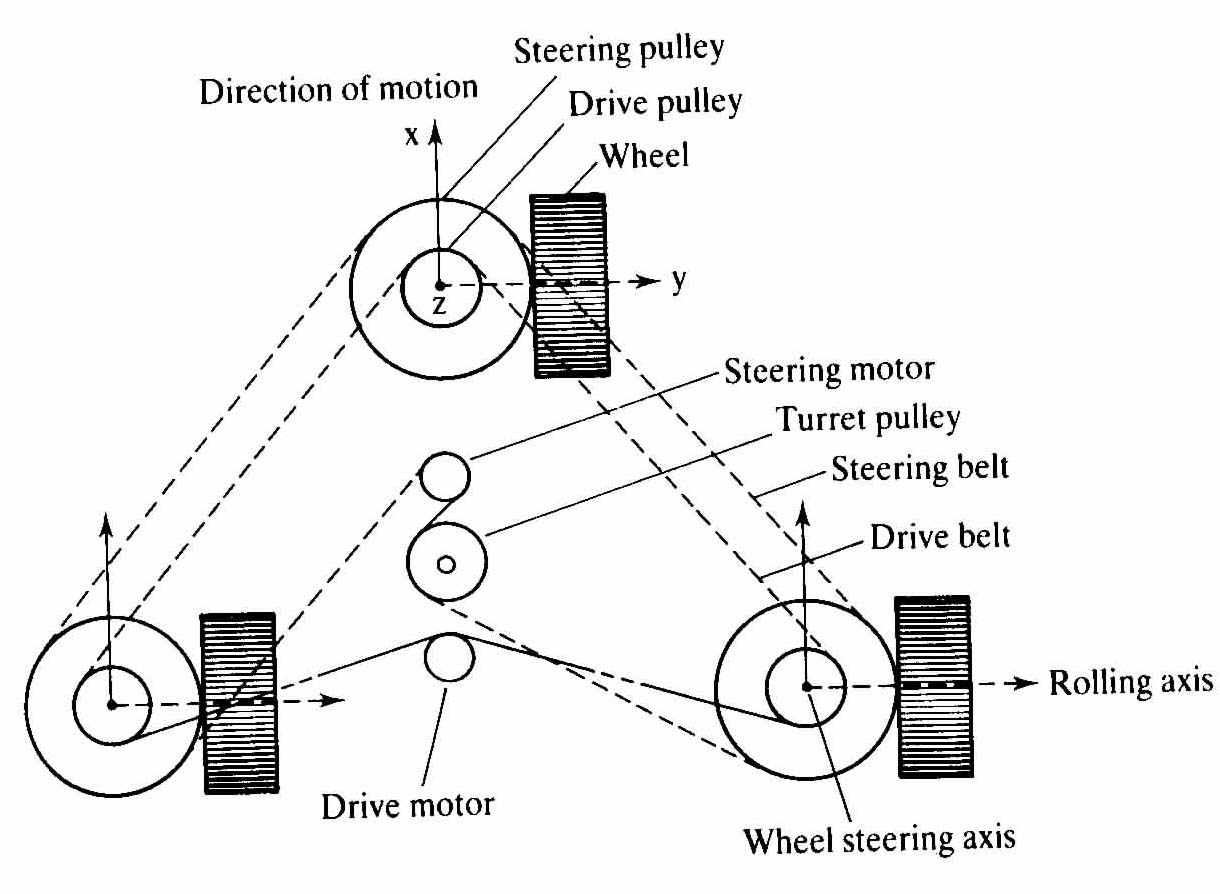
\includegraphics[width=1\textwidth]{mecanismo_interno}
\end{figure}

Este modelo tiene como ventajas la separación de motores entre traslación y rotación que facilita el control, la garantía de control en trayectorias rectilíneas debido a la mecánica del mismo y la facilidad que incluyen las restricciones homólogas que posee. Como desventaja encontramos el complejo diseño mecánico que posee para poder transmitir la rotación y traslación a las tres ruedas simultáneamente y, por ende, su difícil implementación en la realidad.\\
% SEGUIR HABLANDO DE MOVIDAS TEORICAS UN PSEUDO LARGO TRECHO ETC ETC ETC ETC



\section{Análisis cinemático}
	\subsection{Obtención del modelo cinemático directo y su Jacobiano}
	
	Gracias a la mecánica del modelo síncrono, los cálculos para la obtención del modelo cinemático del mismo van a ser muy sencillos, ya que se trata de un modelo con restricciones holónomas, es decir, el comportamiento del vehículo se puede representar a través de sus variables generalizadas ($x$ e $y$ como coordenadas del centro del robot en el plano del suelo y $\varphi$ como la rotación producida frente al estado inicial, es decir, cuando éste vale cero) y la variable temporal y puede ser integrable, simplificando el cálculo.\\
	
	Para el modelo cinemático directo en cuestión, sólo se necesita como dato el valor del radio de las ruedas, $R$, para poder realizar la conversión entre velocidad angular y velocidad lineal. En este trabajo, siendo el grupo de trabajo número 11, se tiene cómo radio de las ruedas el valor de $R = 0.4 m$. Con esto ya se puede hallar el modelo cinemático del robot:\\
	
	Para comenzar se deben detectar las variables generalizadas y de actuación del sistema, respectivamente:
		$$
		q=
		\begin{bmatrix}
		x\\y\\\varphi
		\end{bmatrix}
		$$		
		{\centering y \par}
		$$
		p=
		\begin{bmatrix}
		\dot{\theta}\\\omega
		\end{bmatrix}
		$$

	Como ya se sabe de clase, las variables generalizadas son las que dan información sobre el estado del robot, ya que se encuentran en ellas las coordenadas cartesianas $x$ e $y$ del plano del centro del robot y el ángulo de giro $\varphi$ con respecto al eje X, como se ha decidido definir en este proyecto. Así mismo, las variables de actuación son, como dice su nombre, las variables que reflejarán el valor de movimiento de los motores del robot, es decir, del motor de desplazamiento (velocidad angular $\dot{\theta}$) y el de rotación (velocidad angular $\omega$).\\
	
	Una vez detectadas las variables del sistema, se debe encontrar la relación entre ellas y así conseguir la expresión del Jacobiano:\\
	
	Primero, se define $v$ como la componente global de velocidad de desplazamiento, por lo que se calculará como $v^2=\dot{x}^2+\dot{y}^2$ o como $v=R \dot{\theta}$ y, a su vez, la componentes cartesianas de la velocidad se definirán como\par
	
	{\centering $\dot{x}=v cos(\varphi)$\par} {\centering $\dot{y}=v sin(\varphi)$\\}
	
		
	Sabiendo además que la velocidad de rotación $\dot{\varphi}$ concuerda con la variable de actuación $\omega$, se puede montar la matriz Jacobiana del sistema tal que:
		$$
		J=
		\begin{bmatrix}
			R cos(\varphi) && 0\\
			R sin(\varphi) && 0\\
			0 && 1
		\end{bmatrix}
		$$

	La matriz Jacobiana describirá la cinemática directa del sistema relacionando las variables de actuación con las derivadas de las variables generalizadas y, como se sabe que serán integrables debido a la existencia de restricciones holónomas, se podrán integrar para poder hallar los valores de posición y orientación.\\
	
	Dicho esto, se puede expresar el modelo cinemático como función de entradas (variables de actuación) y salidas (variables generalizadas):
	
		$$
		\begin{bmatrix}
		\dot{x}\\\dot{y}\\\dot{\varphi}
		\end{bmatrix}
		=
		\begin{bmatrix}
		R cos(\varphi) && 0\\
		R sin(\varphi) && 0\\
		0 && 1
		\end{bmatrix}
		\begin{bmatrix}
		\dot{\theta}\\\omega
		\end{bmatrix},
		$$

	e integrando,
	
		$$
		\begin{bmatrix}
		x\\y\\\varphi
		\end{bmatrix}
		=
		\begin{bmatrix}
		x_0\\y_0\\\varphi_0
		\end{bmatrix}
		+
		\begin{bmatrix}
		\int_{0}^{t} R\dot{\theta}cos(\varphi)dt\\
		\int_{0}^{t} R\dot{\theta}sin(\varphi)dt\\
		\int_{0}^{t} \omega dt
		\end{bmatrix},
		$$
	
	siendo $x_0$, $y_0$ y $\varphi_0$ las condiciones iniciales de posición y orientación.\\

	Una vez obtenido el modelo cinemático directo se pueden realizar pruebas para comprobar el correcto funcionamiento del modelo. Para ello se ha utilizado el siguiente script de MATLAB:
	
	\begin{itemize}
		\item \textbf{Pruebas de Modelo Cinemático Directo} 
		\lstset{language=Matlab,columns=flexible,keepspaces=true}
		
			\begin{lstlisting}[frame=single]
			selection='Seleccione el tipo de trayectoria a implementar:\n 0.Lineal/Curva. \n 1.Senoidal.\n';
			sel=input(selection);
			while (sel >1) 
			disp('Error. Parametro no valido\n') 
			selection='Seleccione el tipo de trayectoria a implementar:\n 0.Lineal/Curva. \n 1.Senoidal.\n';
			sel=input(selection);
			end
			
			%%%%%%% Posicion inicial del robot %%%%%%%
			pos_init=[0;0;0];
			
			%%%%%%% Tiempo de simulacion %%%%%%%
			t_sim=30;
			
			%%%%%% Saturacion en velocidades angulares y lineales %%%%%%
			omega_sat=[-0.2618 0.2618];     % 15 grados/segundo
			tetha_d_sat=[-0.75 0.75];       % Velocidad lineal de 30 cm/seg
			
			%%%%%%%% SELECTION DEL TIPO DE TRAYECTORIA DESEADA %%%%%%%%%%
			switch(sel)
			% SI SE DESEA QUE EL ROBOT SIGA UNA TRAYECTORIA LINEAL
			case 0
			selection='Asigne velocidad de giro del robot\n';
			omega=input(selection);
			if omega>omega_sat(2)
			omega=omega_sat(2);
			disp('Valor por encima de la saturacion superior. Se asignara el valor maximo posible')
			elseif omega<omega_sat(1)
			omega=omega_sat(1);
			disp('Valor por debajo de la saturacion inferior. Se asignara el valor minimo posible')
			end
			
			selection='Asigne velocidad de rotacion de las ruedas\n';
			tetha_d=input(selection);
			if tetha_d>tetha_d_sat(2)
			tetha_d=tetha_d_sat(2);
			disp('Valor por encima de la saturacion superior. Se asignara el valor maximo posible')
			elseif tetha_d<tetha_d_sat(1)
			tetha_d=tetha_d_sat(1);
			disp('Valor por debajo de la saturacion inferior. Se asignara el valor minimo posible')
			end
			% Para evitar errores, se inicializan a cero el resto de variables
			freq=0; ampl_sin=0;
			
			% SI SE DESEA QUE EL ROBOT SIGA UNA TRAYECTORIA SENOIDAL
			case 1
			% Parametros senoides
			selection='Asigne frecuencia de la senoide\n';
			freq=input(selection); %Frecuencia de la senoide en la direccion
			selection='Asigne amplitud de la senoide\n';
			ampl_sin=input(selection); %Amplitud de la senoide en la direccion
			
			selection='Asigne velocidad de rotacion de las ruedas\n';
			tetha_d=input(selection);
			if tetha_d>tetha_d_sat(2)
			tetha_d=tetha_d_sat(2);
			disp('Valor por encima de la saturacion superior. Se asignara el valor maximo posible')
			elseif tetha_d<tetha_d_sat(1)
			tetha_d=tetha_d_sat(1);
			disp('Valor por debajo de la saturacion inferior. Se asignara el valor minimo posible')
			end
			% Para evitar errores, se inicializan a cero el resto de variables
			omega=0;
			end
			
			
			% Se lanza la simulacion
			sim('sl_MCD_sincrono');
			
			% Se grafica el resultado obtenido
			figure();hold on;...
			comet(posx,posy);grid; title(' Movimiento del robot en el plano XY');...
			xlabel('Coordenada X del movimiento'); ylabel('Coordenada Y del movimiento');...
			legend('Movimiento del robot','Location','BestOutside');
			% Graficamos el vector velocidad en cada pto de la trayectoria
			plot(posx,posy,'LineWidth',2);
			u=cos(ang_phi);
			v=sin(ang_phi);
			quiver(posx,posy,u,v,'c'); %Ploteo del vector de la velocidad Lineal.
			hold off;
			\end{lstlisting} 
	\end{itemize}

	Con este código se pueden realizar varios experimentos. Para todos ellos las características comunes serán que partirán de las mismas condiciones iniciales para las variables generalizadas ($x=0, y=0, \varphi=0$) y tendrán las mismas saturaciones, que se corresponden, como aparece comentado en el código anterior, a una velocidad lineal de desplazamiento máxima de 30 cm/segundo y una velocidad de rotación máxima de 15 grados/segundo, los cuales hemos supuesto como realistas para este tipo de robot.\\
	
	El primer experimento que se va a mostrar es el de una velocidad de desplazamiento máxima y velocidad de rotación nula. Como la simulación dura 30 segundos, el robot deberá recorrer una distancia de 9 metros:
	
	\begin{figure}[H]
		\centering
		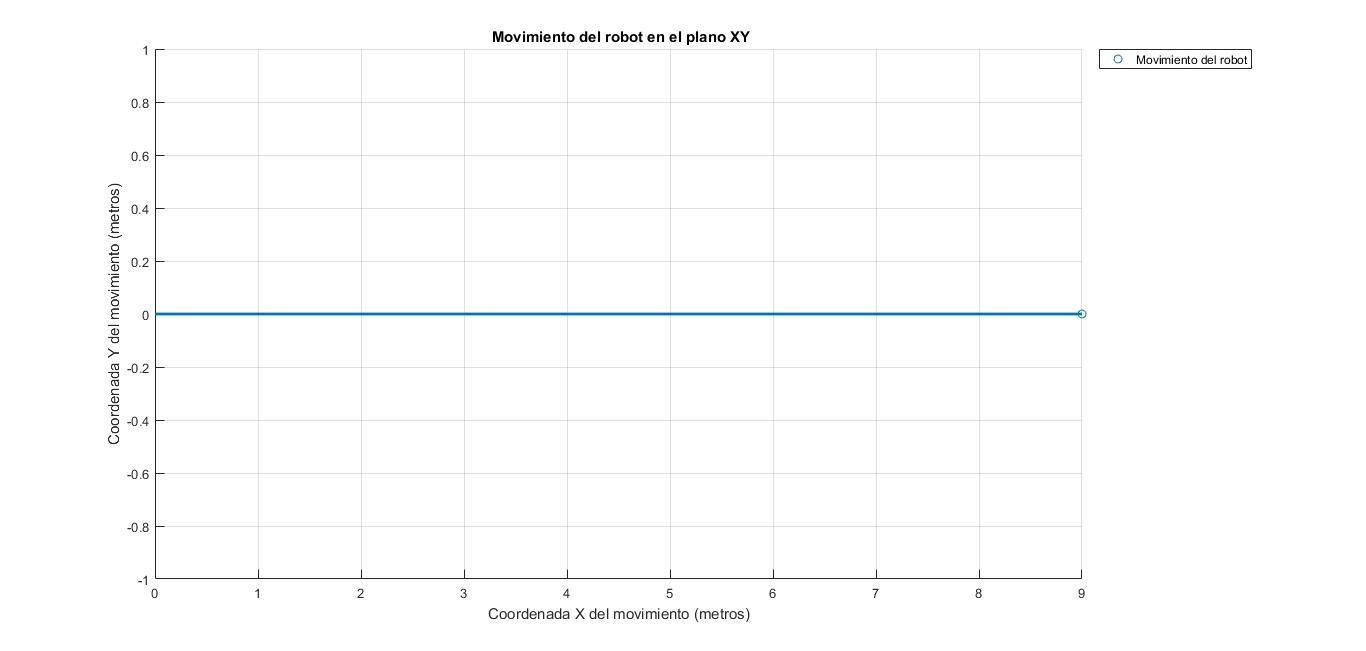
\includegraphics[width=1\textwidth]{exp_MCD_1}
		\caption{Movimiento en el plano con actuación de desplazamiento constante y rotativa nula}
	\end{figure}

	El siguiente experimento combinará ambas variables de actuación, estableciendo el valor máximo en ambas, por lo que el robot deberá dar vueltas en círculo. Como la velocidad de rotación máxima es de 15 grados/segundo y la simulación dura 30 segundos, el robot deberá dar 1 vuelta y 1/4 de vuelta más. En este y el siguiente experimento, al no constar únicamente de una trayectoria rectilínea, se ha aprovechado para representar, a través de flechas, el vector velocidad de desplazamiento:
	
	\begin{figure}[H]
		\centering
		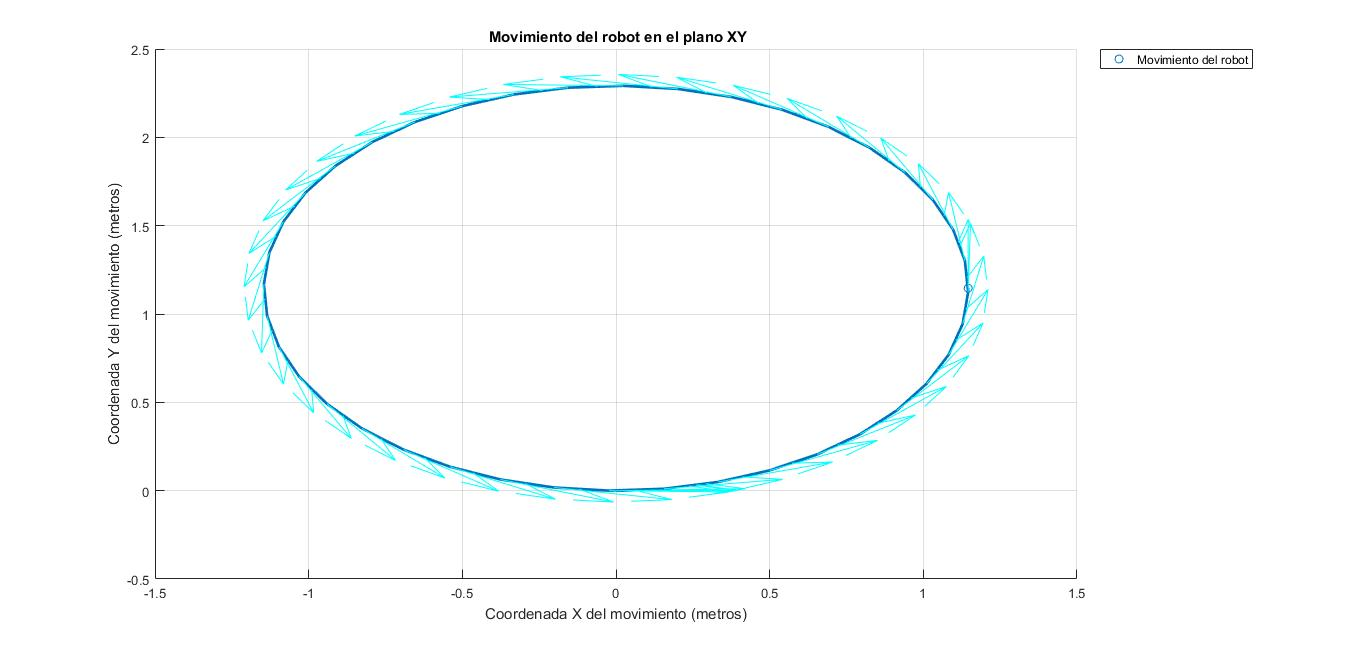
\includegraphics[width=1\textwidth]{exp_MCD_2}
		\caption{Movimiento en el plano con actuación de desplazamiento y rotativa constantes}
	\end{figure}

	Ahora se va a realizar el experimento correspondiente a la prueba solicitada para el trabajo donde se ha de administrar una velocidad de desplazamiento constante y una velocidad de rotación con carácter senoidal. Para ello, se ha introducido una velocidad de desplazamiento de 0.5 radianes/segundo y una senoide de 0.05 Hz de frecuencia y 0.2 radianes/segundo de amplitud:
	
	\begin{figure}[H]
		\centering
		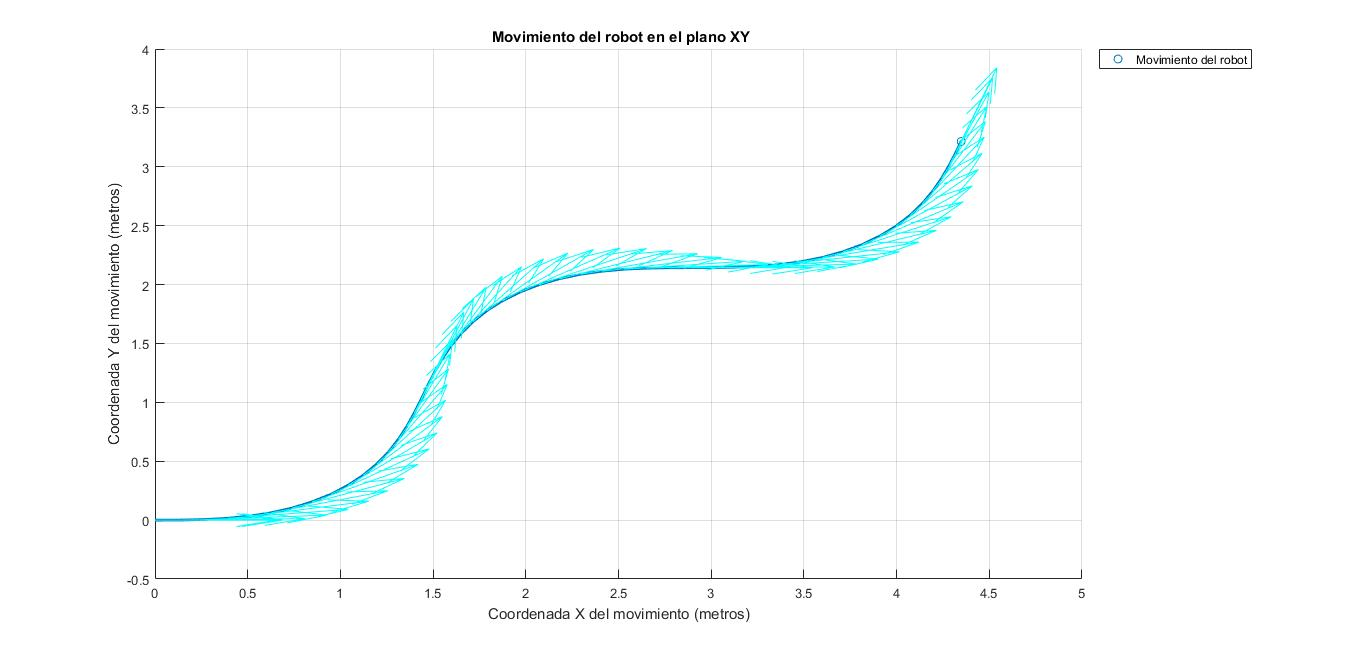
\includegraphics[width=1\textwidth]{exp_MCD_3_1}
		\caption{Movimiento en el plano con actuación rotativa senoidal}
	\end{figure}

	\begin{figure}[H]
		\centering
		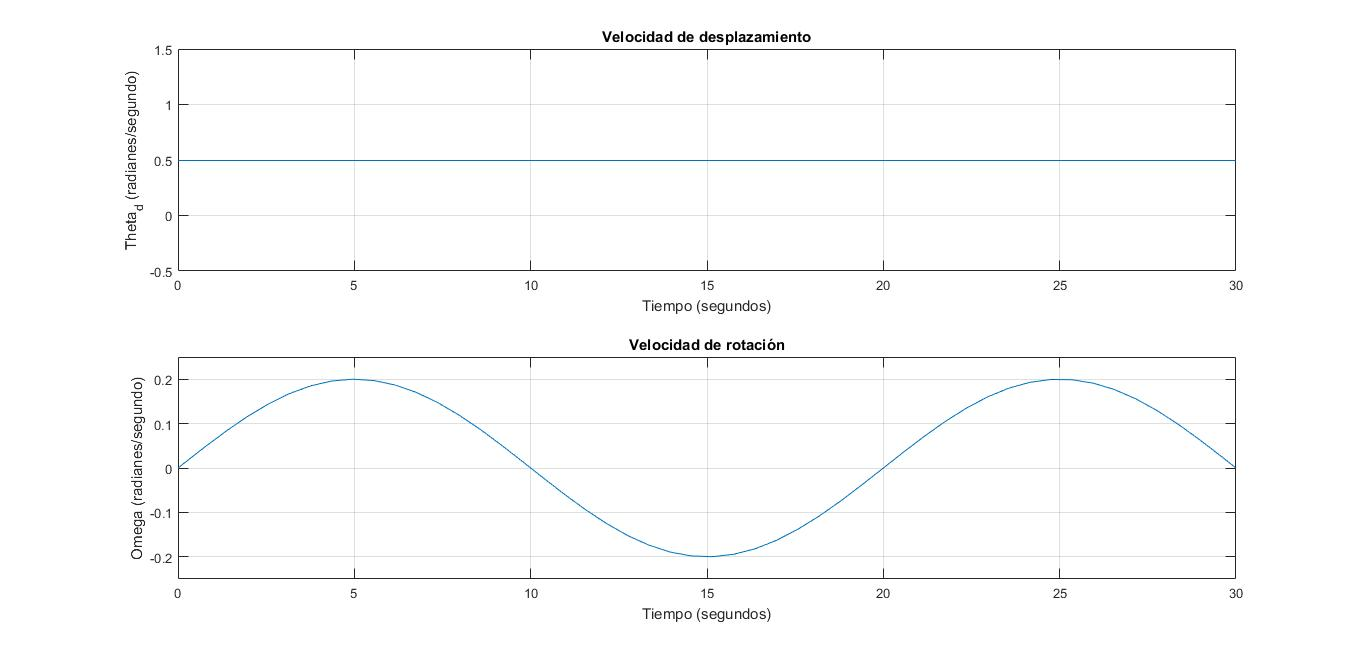
\includegraphics[width=1\textwidth]{exp_MCD_3_2}
		\caption{Variables de actuación tras saturación (arriba $\dot{\theta}$ y abajo $\omega$)}
	\end{figure}

	En este último experimento se puede observar que la variable de actuación $\omega$ (figura 4, gráfica inferior) resulta ser la senoide esperada y que, como resultado, se obtiene también una trayectoria senoidal (figura 3).\\

	Para finalizar esta sección, se mostrará el montaje en Simulink que ha sido utilizado para obtener los resultados:
	
	\begin{figure}[H]
		\centering
		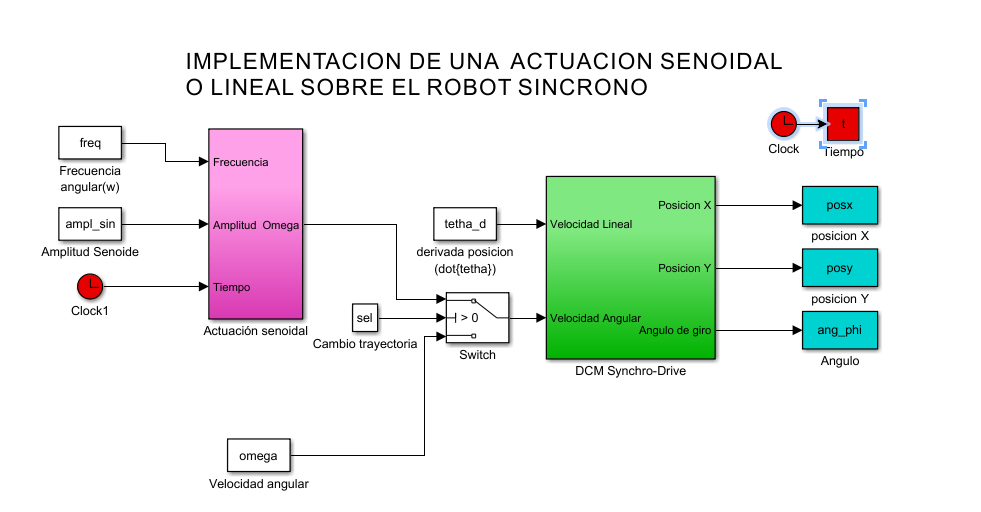
\includegraphics[width=1.1\textwidth]{simulink_MCD_1}
		\caption{Esquema global}
	\end{figure}

	\begin{figure}[H]
		\centering
		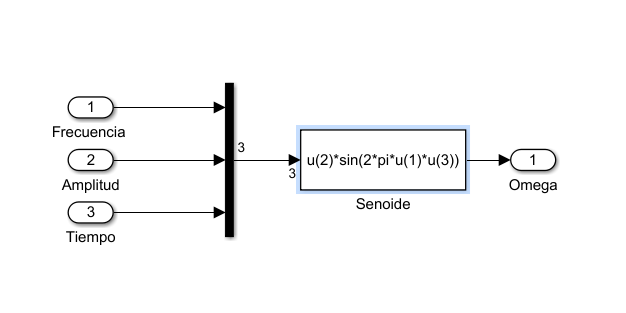
\includegraphics[width=1\textwidth]{simulink_MCD_2}
		\caption{Esquema del bloque "Actuación Senoidal"}
	\end{figure}

	\begin{figure}[H]
		\centering
		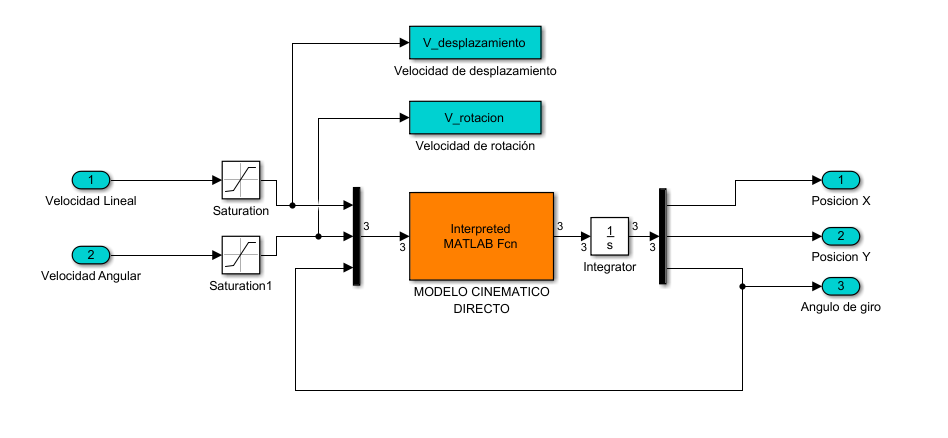
\includegraphics[width=1.2\textwidth]{simulink_MCD_3}
		\caption{Esquema del bloque "DCM Synchro-Drive"}
	\end{figure}

	Dentro del bloque "Interpreted MATLAB Fcn" del esquema de la figura 7 se encuentra la función que contiene el modelo cinemático directo del robot, la cual sigue la siguiente estructura:
	
	\begin{itemize}
		\item \textbf{Función de Modelo Cinemático Directo} 
		\lstset{language=Matlab,columns=flexible,keepspaces=true}
		
		\begin{lstlisting}[frame=single]
		function gener_out=MCD_movil(in) 
		R=0.4; %-> Radio de la rueda [m]
		
		
		tetha_d=in(1);  % Velocidad de desplazamiento
		omega=in(2);    % Velocidad de rotacion
		phi=in(3);      % Angulo del robot
		
		% Jacobiano de velocidades
		jac=[R*cos(phi) 0;
		R*sin(phi) 0;
		0       1];
		
		% Vector de variables actuadoras de entrada
		act=[tetha_d;
		omega];
		
		% Definicion de salidas
		x_d=jac(1,:)*act;
		y_d=jac(2,:)*act;
		phi_d=jac(3,:)*act;
		
		gener_out=[x_d;y_d;phi_d];
		end
		\end{lstlisting} 
	\end{itemize}


	\subsection{Obtención del modelo cinemático inverso}
	
	Una vez comentado todo lo que concierne a la cinemática directa, se puede pasar a obtener el modelo cinemático inverso, el cual será de utilidad para la creación de trayectorias con las variables generalizadas y su posterior transformación a variables de actuación que harán que el robot siga dicha trayectoria.\\
	
	Dicho esto, el modelo cinemático inverso se basa principalmente en la Jacobiana inversa, ya que ahora se desea relacionar las variables generalizadas como entradas con las variables de actuación como salida. Por ello únicamente hay que coger la ecuación del modelo cinemático directo y pasar el Jacobiano al otro lado, es decir, poner su inversa. \\
	
	En este caso se da que el Jacobiano del modelo directo no es una matriz cuadrada, por lo que no puede tener inversa, así que habrá que realizar la pseudoinversa del mismo. Para ello, no es necesario realizar los cálculos paso por paso, ya que MATLAB posee una función que calcula la pseudoinversa por el método Moore-Penrose llamada $pinv$. Dicho esto, una vez utilizada la función y habiendo simplificado, el resultado es:
	
	$$
		J^{-1}=
		\begin{bmatrix}
		cos(\varphi)/R && sin(\varphi)/R && 0\\
		0 && 0 && 1
		\end{bmatrix}
	$$
	
	Una vez obtenida la expresión del Jacobiano inverso, simplemente bastaría con introducirle los datos de entrada necesarios ($\dot{x}$, $\dot{y}$ y $\dot{\varphi}$) para obtener las salidas esperadas ($\dot{\theta}$ y $\omega$).\\
	
	Para garantizar el funcionamiento del modelo inverso, se va a realizar el tercer apartado del proyecto, donde se pide obtener las señales de control necesarias para que el robot realice una trayectoria parabólica, la cual va a venir dada por la expresión:\\ $$y=-x(x-A)/D,$$
	
	donde, $x$ e $y$ son las coordenadas cartesianas de la posición del centro del robot, $A$ una constante que determinará el valor máximo en $x$ que alcanzará la parábola y $D$ otra constante que determinará el valor máximo en $y$ que alcanzará la parábola.\\
	
	Para explicar como se ha llevado a cabo el proceso de obtención de los resultados, se va a hacer uso del montaje en Simulink utilizado en esta parte:
	
	\begin{figure}[H]
		\centering
		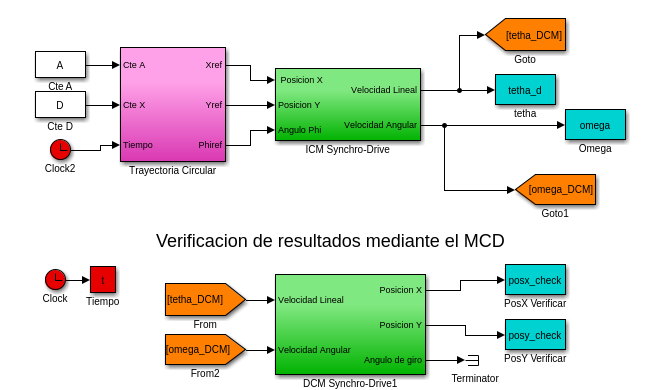
\includegraphics[width=1\textwidth]{simulink_MCI_1}
		\caption{Esquema global}
	\end{figure}
	
	Dado el esquema global utilizado para la simulación del experimento, se va a empezar a explicar en orden de ejecución, por lo que se comenzará por el bloque de "Trayectoria Parabólica":
	
	\begin{figure}[H]
		\centering
		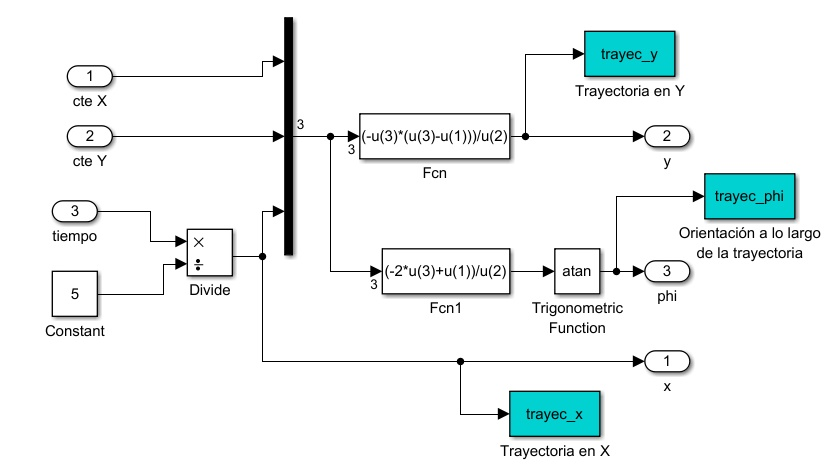
\includegraphics[width=1\textwidth]{simulink_MCI_2}
		\caption{Bloque de Trayectoria Parabólica}
	\end{figure}

	Como se pudo observar, las entradas a este bloque son las 2 constantes ($A$ y $D$) de la parábola y el tiempo de simulación. Las dos primeras son utilizadas para la formulación de la parábola en sí y la tercera para la definición de $x$, que crecerá linealmente pero a una escala 5 veces más pequeña que el tiempo de simulación.\\
	
	A la derecha del multiplexor se encuentra una primera función que determinará el valor de $y$, es decir, es la función de la parábola, tal y como se había descrito anteriormente.\\
	
	Un poco más abajo se encuentra otra función que en realidad la derivada de la primera, puesto que se busca calcular la tangente a la parábola en cada instante para así poder obtener la pendiente de dicha recta, realizar la arcotangente y hallar el ángulo que conforma con el eje X, que coincidirá con la definición del ángulo $\varphi$.\\
	
	Una vez se han definido los puntos de la trayectoria que ha de seguir el robot y con qué orientación ha de hacerlo, simplemente hay que pasar dichos datos al bloque donde se encuentra el modelo cinemático inverso:
	
	\begin{figure}[H]
		\centering
		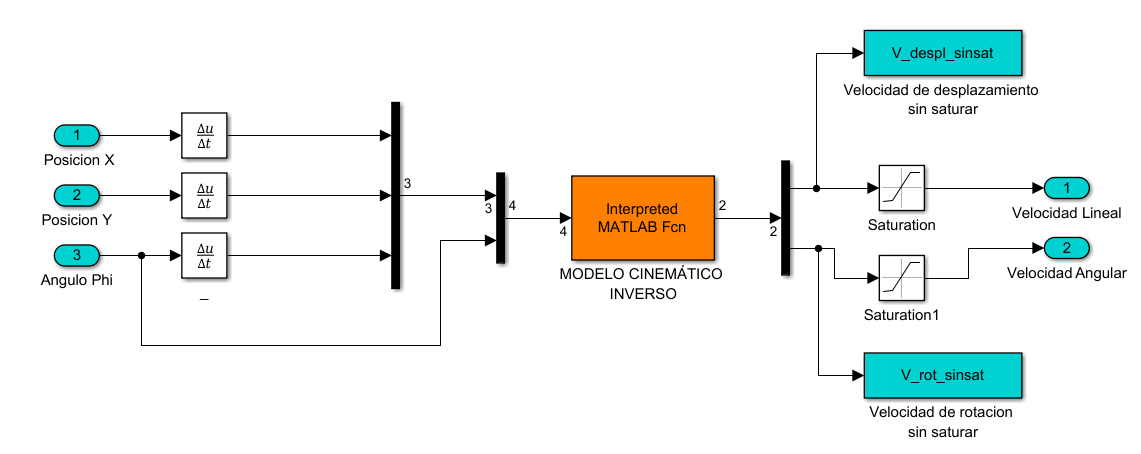
\includegraphics[width=1\textwidth]{simulink_MCI_3}
		\caption{Bloque ICM Synchro-Drive}
	\end{figure}

	Como se puede observar, lo primero que se debe hacer es derivar cada una de las entradas respecto al tiempo, puesto que el Jacobiano inverso, como antes lo hacía el directo, considera relaciones entre velocidades.\\
	
	Una vez hecho eso, se introducen los valores en el bloque que contiene a la función que ejecuta la cinemática inversa, cuyo código es el siguiente:
	
	\begin{itemize}
		\item \textbf{Función de Modelo Cinemático Inverso} 
		\lstset{language=Matlab,columns=flexible,keepspaces=true}
		
		\begin{lstlisting}[frame=single]
		function gener_out=MCI_movil(in)
		R=0.4; %-> Radio de la rueda [m]
		
		
		x_d=in(1);  % Velocidad cartesiana X
		y_d=in(2);    % Velocidad cartesiana Y
		phi_d=in(3);      % Velocidad angular phi
		phi=in(4);      % Angulo phi
		
		% Jacobiano inverso de velocidades
		jac_inv=[cos(phi)/R, sin(phi)/R, 0;
			          0,          0, 1];
		
		%Vector de parametros generalizados
		gen=[x_d y_d phi_d]';
		
		
		% Definicion de salidas
		tetha_d=jac_inv(1,:)*gen;
		omega=jac_inv(2,:)*gen;
		
		gener_out=[tetha_d;omega];
		end
		\end{lstlisting} 
	\end{itemize}

	Se observa que simplemente se realiza la multiplicación matricial para obtener las variables de actuación.\\
	
	Por último, antes de volver al esquema global, se saturan los valores de estas salidas con las mismas saturaciones que se habían determinado realistas en la cinemática directa.\\
	
	Para terminar, en el esquema global, se coloca de nuevo el bloque de la cinemática directa para comprobar, con las variables de actuación obtenidas con el modelo inverso, se obtiene la misma trayectoria que se ha diseñado.\\
	
	Con el montaje en Simulink ya creado, lo único que falta es lanzar un script que asigne valores a las incógnitas de la simulación ($A$ y $D$) y represente los datos:
	
	\begin{itemize}
		\item \textbf{Prueba de Modelo Cinemático Inverso} 
		\lstset{language=Matlab,columns=flexible,keepspaces=true}
		
		\begin{lstlisting}[frame=single]
		%Tiempo de simulacion
		t_sim=15;
		
		%%%%%%% Posicion inicial del robot %%%%%%%
		pos_init=[0;0;0.2915];%El valor de phi sera el valor del angulo sacado por la arcotangente de la derivada de la parabola en t=0
		
		%%%%%% Saturacion en velocidades angulares y lineales %%%%%%
		omega_sat=[-0.2618 0.2618];     % 15 grados/segundo
		tetha_d_sat=[-0.75 0.75];       % Velocidad lineal de 30 cm/seg
		
		% Descripcion de la entrada parabolica.
		A=3;
		D=10;
		
		% Se lanza la simulacion
		sim('sl_MCI_sincrono');
		
		%Comprobamos Resultado
		figure();
		plot(posx_check,posy_check,'b',trayec_x,trayec_y,'r');grid; title(' Movimiento del robot en el plano XY');...
		xlabel('Coordenada X del movimiento (metros)'); ylabel('Coordenada Y del movimiento (metros)');...
		legend('Movimiento del robot','Location','BestOutside');
		\end{lstlisting} 
	\end{itemize}
	
	Debemos tener en cuenta siempre que en la posición inicial hay que determinar la orientación inicial que debe tener el robot, lo cual se podrá obtener fácilmente como $atan(A/D)$. Esto debe ser así porque, en caso contrario, al estar el robot en reposo con $\varphi$ nulo, al principio de la trayectoria el valor de velocidad de rotación saturará intentando conseguir dicha orientación y la trayectoria no será la misma porque el sistema, con dicha saturación, no será capaz de realizarla en un tiempo tan pequeño. Así, para unos valores de $A=3$ y $D=10$, obtenemos:
	
	\begin{figure}[H]
		\centering
		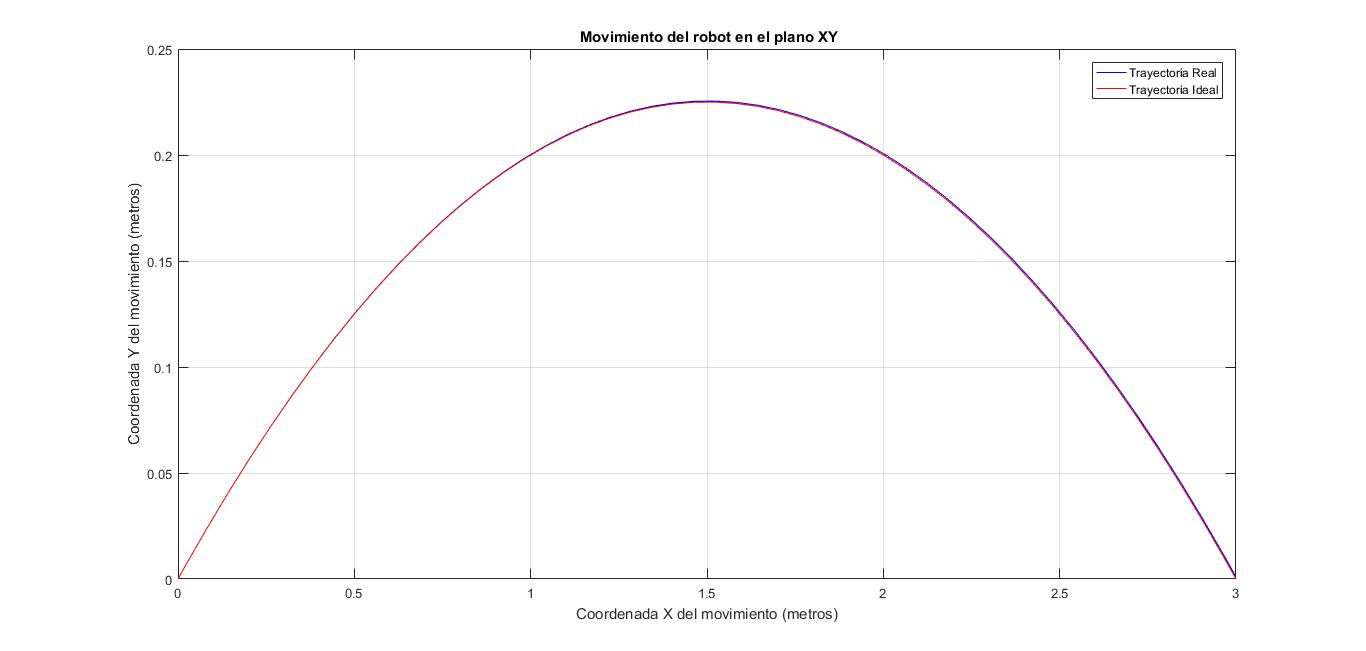
\includegraphics[width=1.1\textwidth]{parab_1}
		\caption{Comparativa entre la trayectoria pedida y la obtenida}
	\end{figure}
	
	Como se puede observar, en la gráfica comparativa anterior entre la trayectoria creada por funciones y la obtenida a partir de los valores de las variables de actuación sacadas del modelo cinemático inverso, los resultados son prácticamente iguales, por lo que se puede decir que el modelo inverso es aceptable.\\
	
	Aparte, se van a mostrar las gráficas de los valores de las variables de actuación obtenidas con la cinemática inversa, así como el valor de la variable $\varphi$:
	
	\begin{figure}[H]
		\centering
		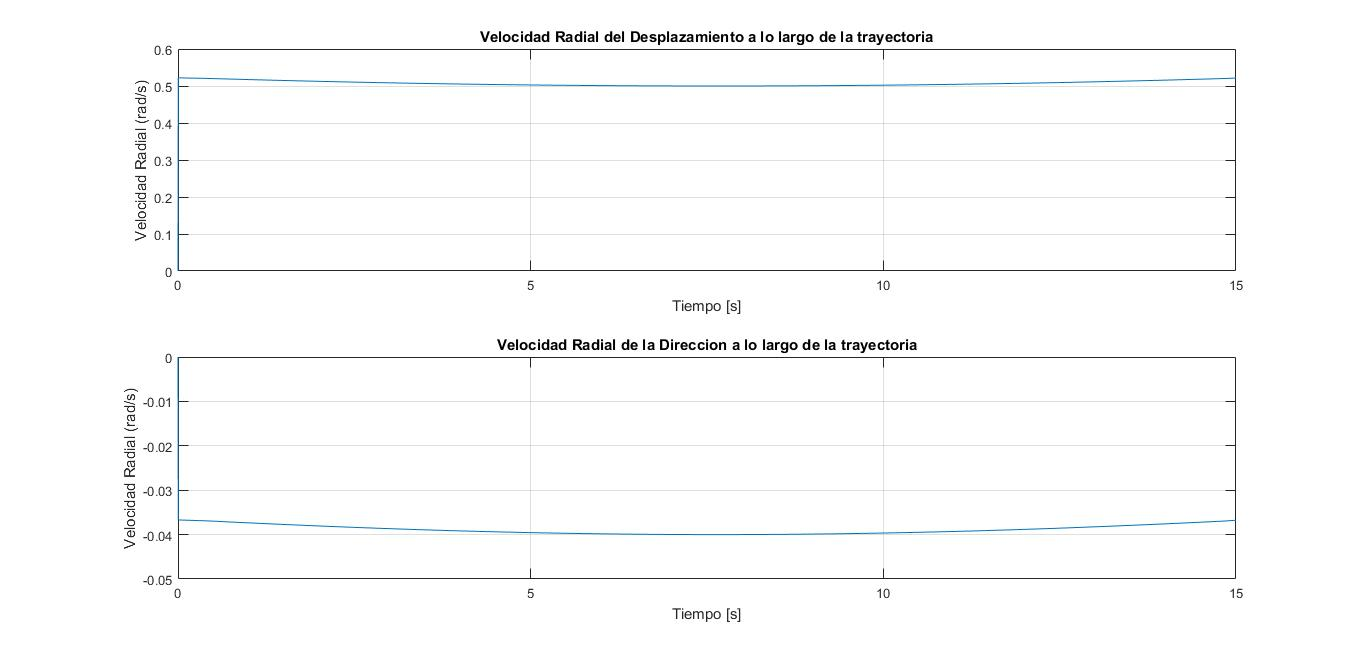
\includegraphics[width=1\textwidth]{parab_2}
		\caption{Valores de las variables de actuación}
	\end{figure}

	\begin{figure}[H]
		\centering
		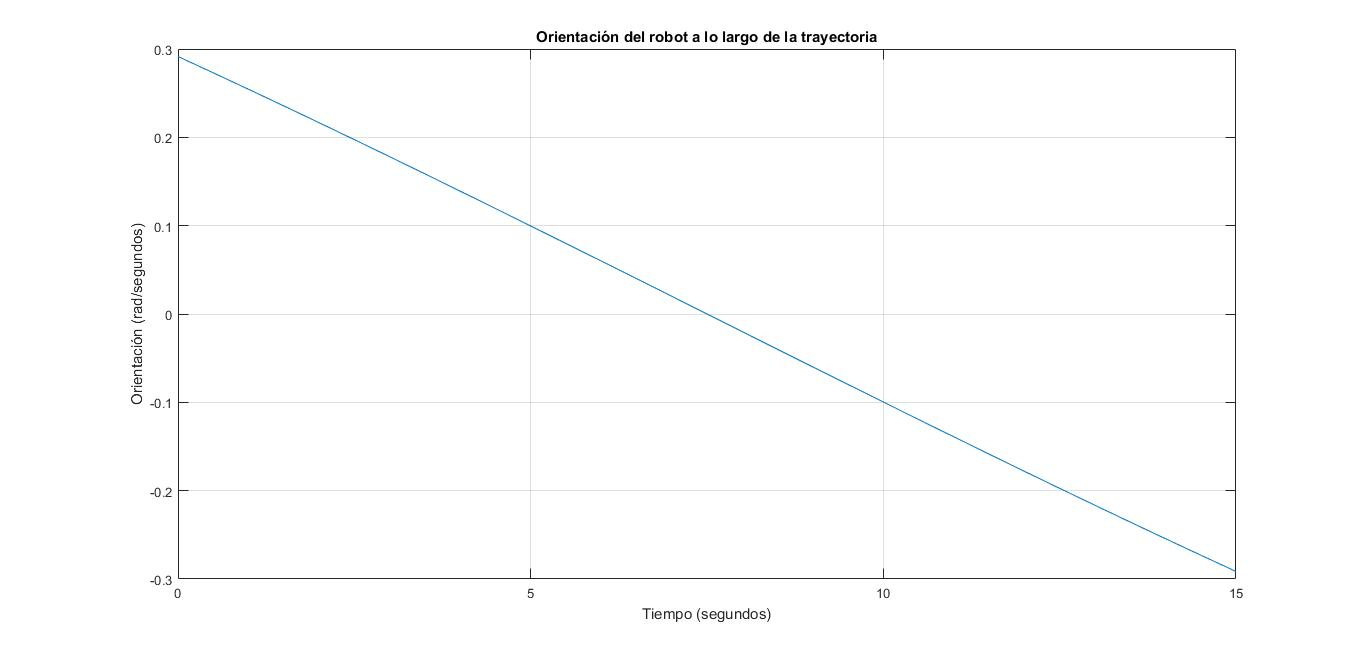
\includegraphics[width=1\textwidth]{parab_3}
		\caption{Valor de la orientación a lo largo de la trayectoria}
	\end{figure}

	Como se observa, en ambas velocidades no se produce saturación alguna, ya que están por debajo y por encima de sus respectivos valores de saturación. Además, con la gráfica de la orientación, se puede observar como justo a la mitad de la trayectoria, la misma es 0, ya que el robot se encuentra en paralelo al eje X en dicho momento.\\
	
	Cabe añadir que es lo que pasaría si las variables de actuación saturasen, ya que no podrían realizar la misma trayectoria. Para ello se van a mostrar dos experimentos distintos. El primero de ellos se basa en bajar la saturación de $\dot{\theta}$ a la mitad, es decir, a $\pm$0.375:
	
	\begin{figure}[H]
		\centering
		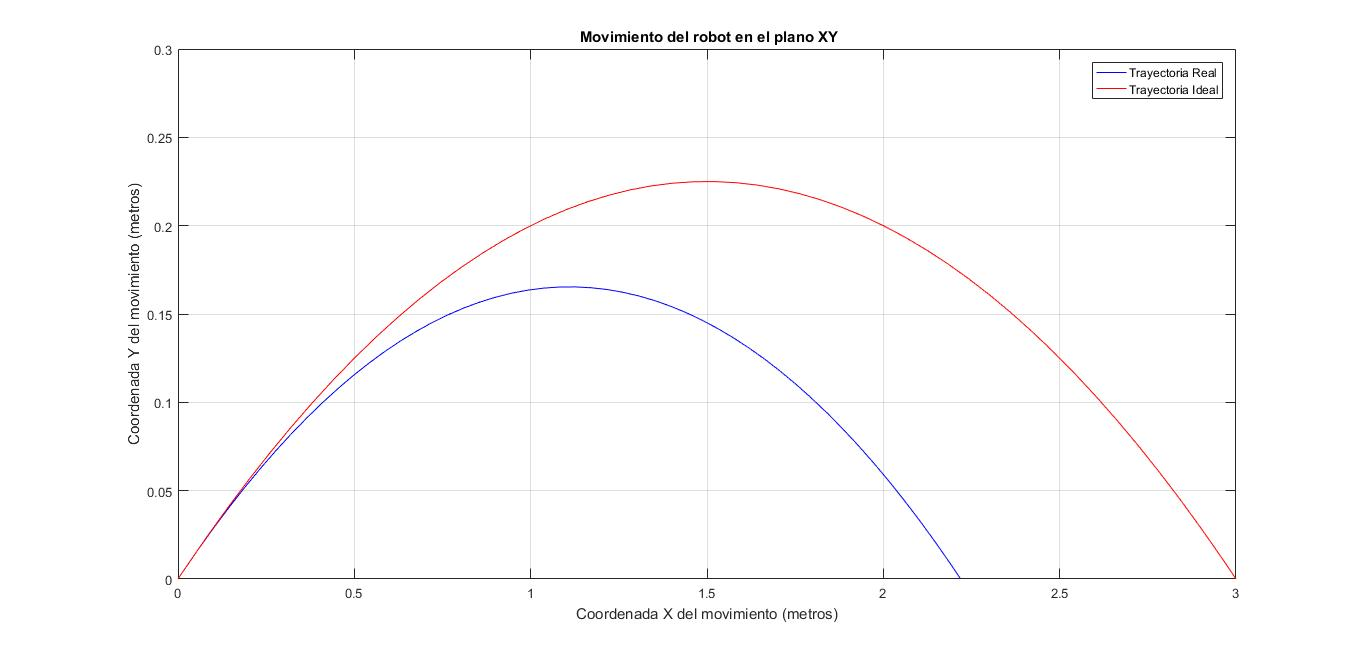
\includegraphics[width=1\textwidth]{parab_4}
		\caption{Comparativa de trayectorias con $\dot{\theta}$ saturada}
	\end{figure}
	
	\begin{figure}[H]
		\centering
		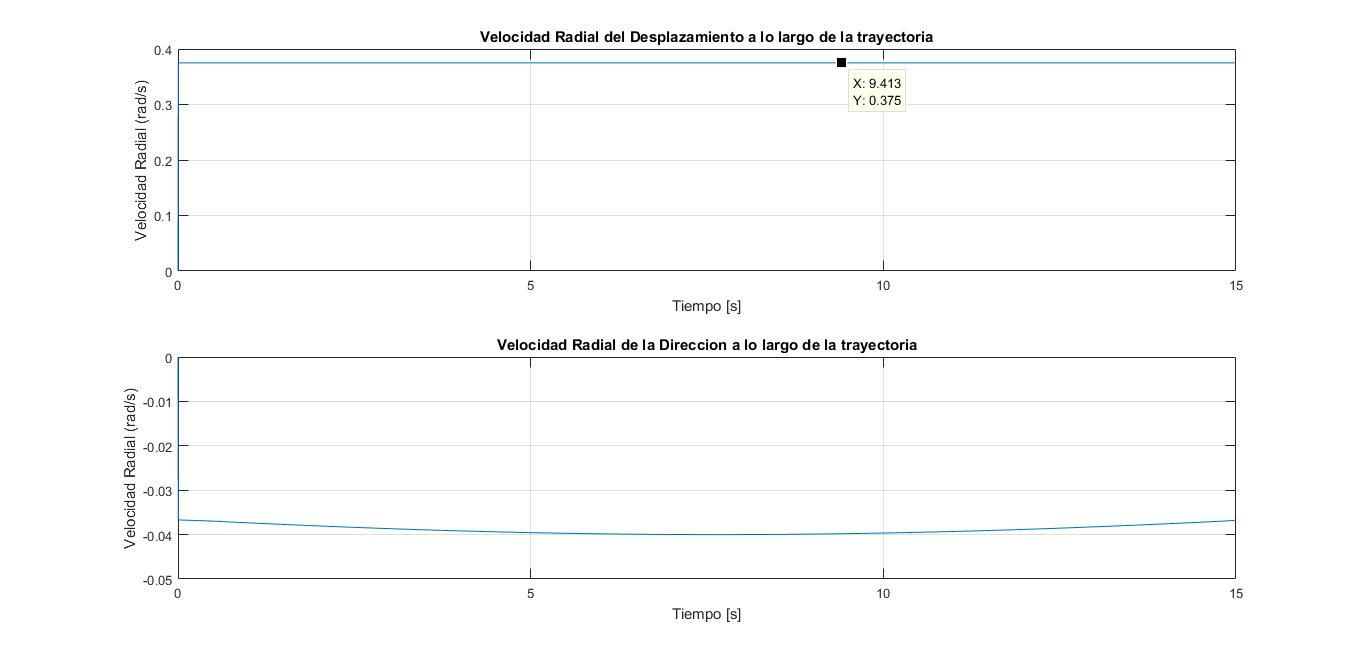
\includegraphics[width=1\textwidth]{parab_5}
		\caption{Valores de variables de actuación con saturación en $\dot{\theta}$}
	\end{figure}
	
	Como se puede observar, la trayectoria real que alcanza el robot se reduce tanto en $x$ como en $y$. Esto es lógico desde el punto de vista de la cinemática, puesto que al no poder alcanzar la velocidad necesaria, no llegará a ninguno de los valores objetivos en las coordenadas cartesianas. En la figura 15 se puede ver como $\dot{\theta}$ satura mientras que $\omega$ no.\\
	
	Ahora se probará a saturar la velocidad de rotación, reduciendo el límite original a una décima parte, obteniendo una nueva saturación de $\pm$0.02618:
	
	\begin{figure}[H]
		\centering
		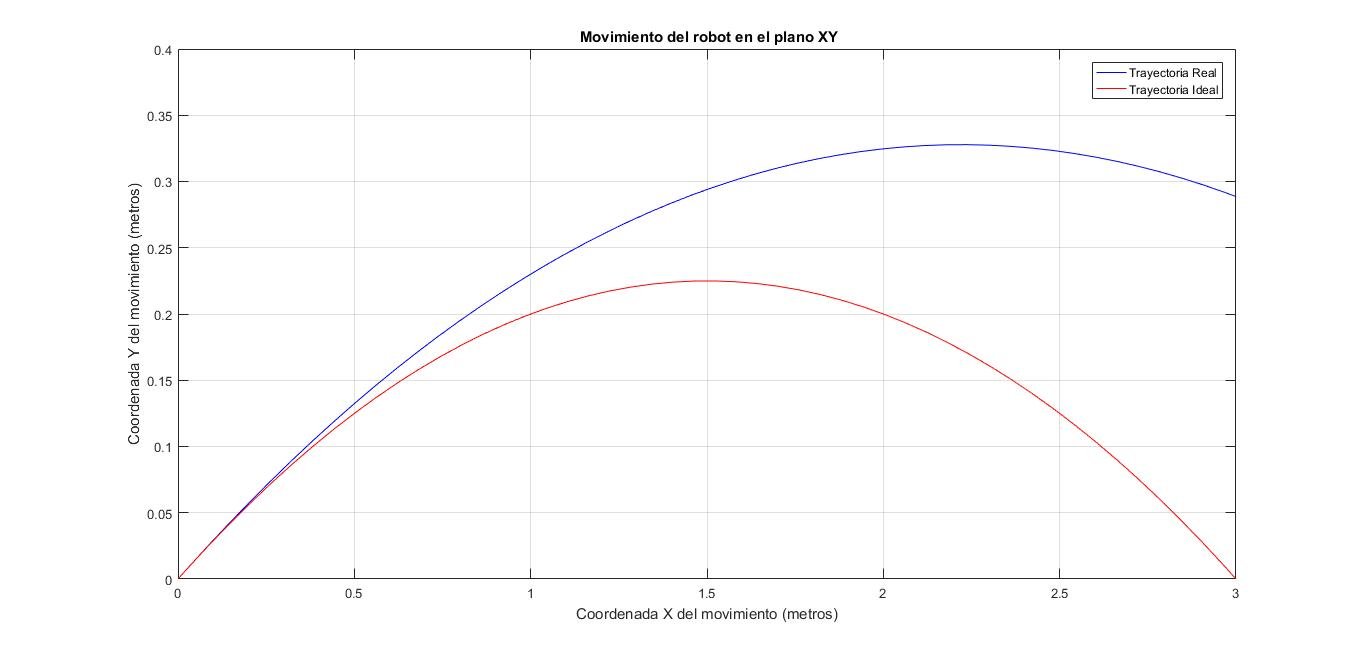
\includegraphics[width=1\textwidth]{parab_6}
		\caption{Comparativa de trayectorias con $\omega$ saturada}
	\end{figure}
	
	\begin{figure}[H]
		\centering
		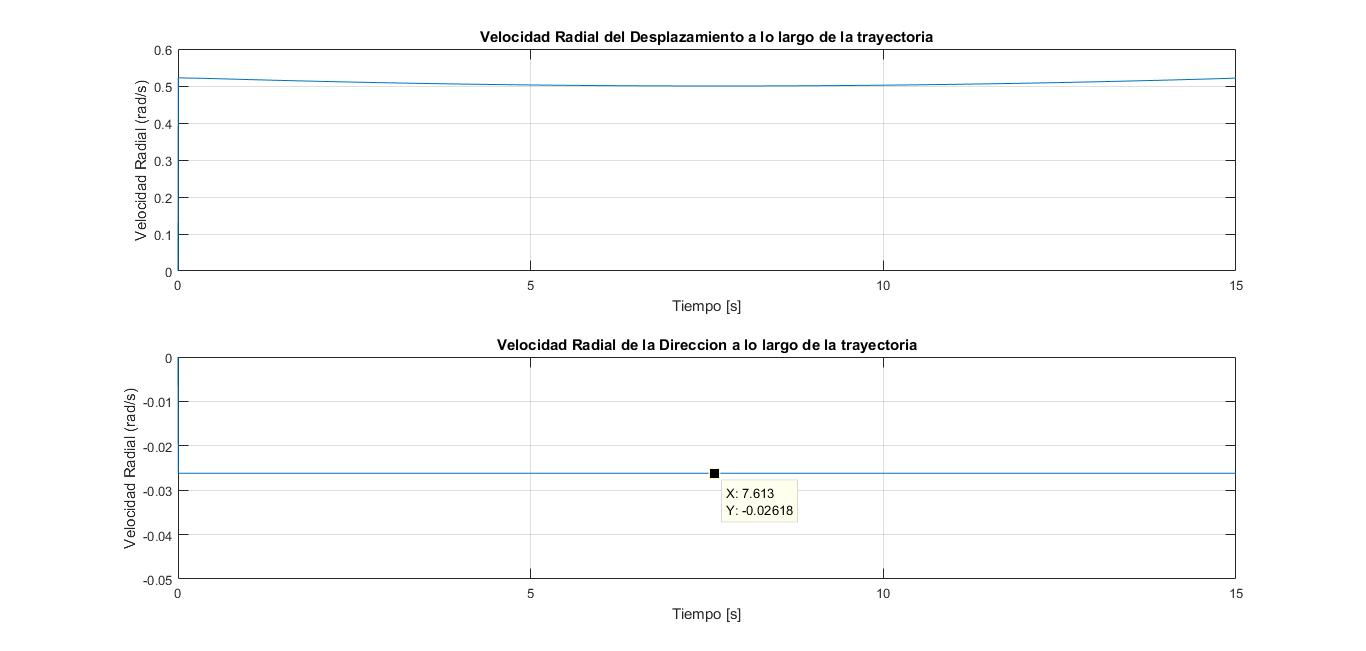
\includegraphics[width=1\textwidth]{parab_7}
		\caption{Valores de variables de actuación con saturación en $\omega$}
	\end{figure}

	Aquí, como también era de esperar, el robot no puede seguir la trayectoria especificada, aunque esta vez lo hace de forma distinta. Esto se debe a que tiene la velocidad de desplazamiento necesaria para alcanzar los puntos objetivos pero no la capacidad de rotar lo suficientemente rápido como para seguirlos y por ello, se sobrepasa de sus objetivos. En la figura 17 se observa la saturación en $\omega$.\\
	
	El efecto que se produce al haber saturaciones en ambas actuaciones es una combinación de ambos resultados, es decir, el "no poder girar a tiempo" y el "no avanzar lo suficientemente rápido":
	
	\begin{figure}[H]
		\centering
		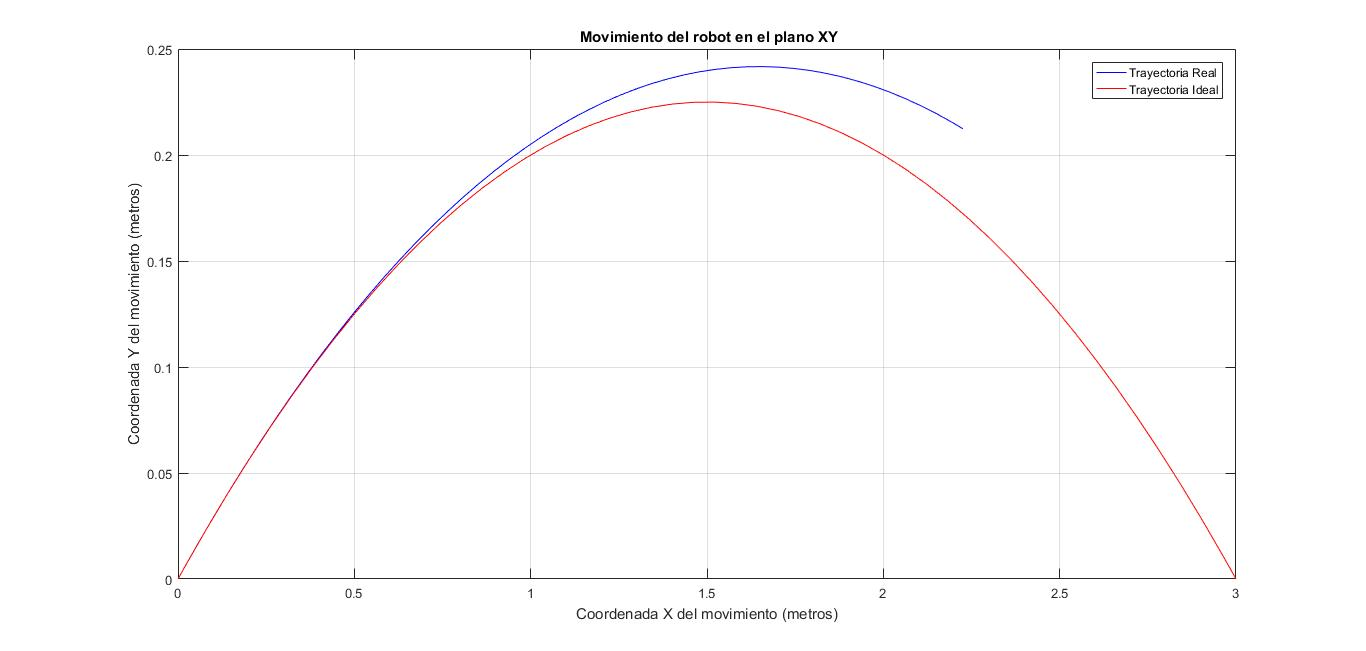
\includegraphics[width=1\textwidth]{parab_8}
		\caption{Comparativa de trayectorias con $\omega$ y $\dot{\theta}$ saturadas}
	\end{figure}
	
	\begin{figure}[H]
		\centering
		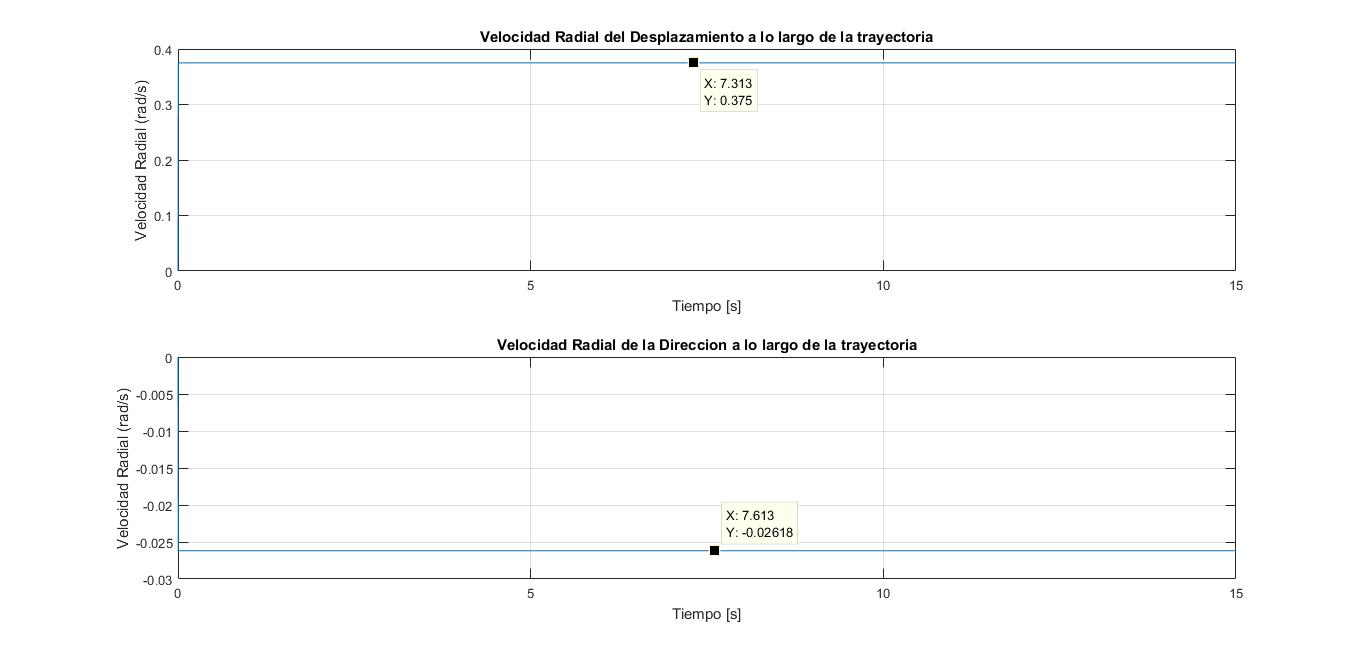
\includegraphics[width=1\textwidth]{parab_9}
		\caption{Valores de variables de actuación con saturación en $\omega$ y $\dot{\theta}$}
	\end{figure}

\section{Control dinámico}
	\subsection{Implementación de diversos algoritmos de control}
		\subsubsection{Control a un punto}
		\subsubsection{Control a una linea}
		\subsubsection{Control a una trayectoria}
		\subsubsection{Control a una postura}
	\subsection{Ley de control \textit{Persecución pura}}

\section{Anexos y conclusiones}
\end{document}
